\documentclass[10pt]{beamer}

\usepackage[utf8]{inputenc}
\usepackage[spanish, es-tabla]{babel}

\usetheme{metropolis}
\usepackage{appendixnumberbeamer}

\usepackage{booktabs}
\usepackage[scale=2]{ccicons}

\usepackage{pgfplots}
\usepgfplotslibrary{dateplot}

\usepackage{caption}
\usepackage{subcaption}

\usepackage{graphicx}

\usepackage[normalem]{ulem}
\useunder{\uline}{\ul}{}

\usepackage{amsmath}
\usepackage{amsfonts}
\usepackage{amssymb}
\usepackage{amsthm}
\usepackage{esvect}

\usepackage{multimedia}

\usepackage[spanish,onelanguage]{algorithm2e} %for psuedo code

\usepackage{xspace}
\newcommand{\themename}{\textbf{\textsc{metropolis}}\xspace}

\title{Detección de anomalías basada en técnicas de ensembles}
\author{Ignacio Aguilera Martos}
\date{\today}
\institute{Trabajo Fin de Grado \\ \href{https://github.com/nacheteam/Ensemble-Outlier-Analysis}{Código disponible en GitHub}}

\begin{document}

\maketitle

\begin{frame}[fragile]{Contenidos}
  \setbeamertemplate{section in toc}[sections numbered]
  \tableofcontents[hideallsubsections]
\end{frame}

\section{Concepto de anomalía basado en distancias}

\begin{frame}[fragile]{Tukey's Fences}
\vspace{10px}
\pause
\metroset{block=fill}

Pensado para el caso uno-dimensional.

\pause

\begin{block}{Tukey's Fences}
	Valores fuera del rango $[Q_1 - k(Q_3 - Q_1), Q_3 + k(Q_3 - Q_1)]$ con $k=1.5$
\end{block}

\pause

La propuesta de $k=1.5$ es arbitraria.

\end{frame}

\begin{frame}[fragile]{Tukey's Fences}
\vspace{10px}
\metroset{block=fill}
\centering
\movie[height = 0.8\textheight, width=0.8\textwidth, poster, showcontrols]{}{Imagenes/outlier-1d.mp4}

\end{frame}

\begin{frame}[fragile]{Tukey's Fences}
\vspace{10px}
\metroset{block=fill}

\begin{figure}
	\centering
	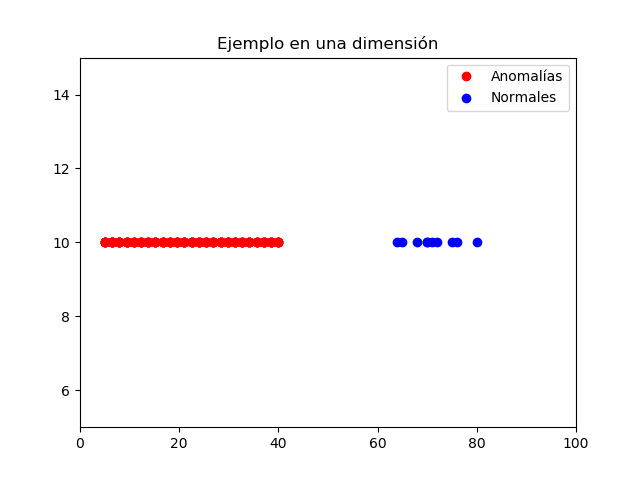
\includegraphics[scale=0.6]{Imagenes/outlier-1d.png}
\end{figure}

\end{frame}

\begin{frame}[fragile]{Extensión al caso de mayor dimensionalidad}
\vspace{10px}
\pause
\metroset{block=fill}

\begin{block}{Criterio}
	Aplicar el criterio de Tukey a cada una de las características.
	\pause
	\textbf{\underline{Trivial}}.
\end{block}

\pause

\begin{block}{Criterio de clusters}
	\begin{enumerate}
		\item Agrupamos los datos por clusters.
		\pause
		\item Encontramos el cluster más cercano para cada instancia.
		\pause
		\item Si la distancia del objeto al centroide del cluster es mayor que $1.5$ veces la mayor
		distancia intercluster entonces es una anomalía.
	\end{enumerate}
\end{block}

\end{frame}

\begin{frame}[fragile]{Ejemplo 1}
\vspace{10px}
\metroset{block=fill}
\centering
\movie[height = 0.8\textheight, width=0.8\textwidth, poster, showcontrols]{}{Imagenes/outlier-2d-case1.mp4}

\end{frame}

\begin{frame}[fragile]{Ejemplo 1}
\vspace{10px}
\metroset{block=fill}

\begin{figure}
	\centering
	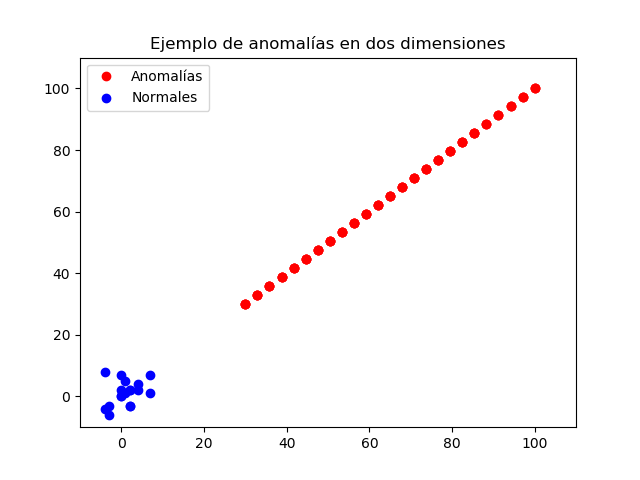
\includegraphics[scale=0.6]{Imagenes/outlier-2d-case1.png}
\end{figure}

\end{frame}

\begin{frame}[fragile]{Ejemplo 2}
\vspace{10px}
\metroset{block=fill}
\centering
\movie[height = 0.8\textheight, width=0.8\textwidth, poster, showcontrols]{}{Imagenes/outlier-2d-case2.mp4}

\end{frame}

\begin{frame}[fragile]{Ejemplo 2}
\vspace{10px}
\metroset{block=fill}

\begin{figure}
\centering
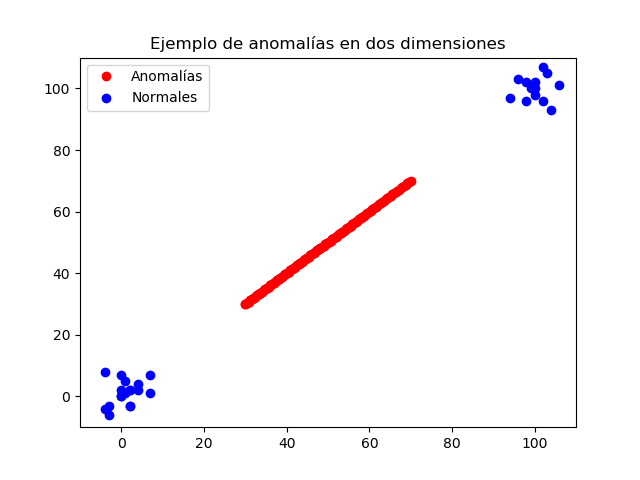
\includegraphics[scale=0.6]{Imagenes/outlier-2d-case2.png}
\end{figure}

\end{frame}

\section{Aprendizaje Automático}

\begin{frame}[fragile]{Problema que abordamos}
\vspace{10px}
\pause
\metroset{block=fill}

\begin{alertblock}{Problema de detección de anomalías}
	Es un problema de aprendizaje no supervisado pues no disponemos de las etiquetas.
\end{alertblock}

\pause

\begin{block}{Partes teóricas del problema}
	\begin{enumerate}
		\item Generador.
		\item Sistema.
		\item Máquina de aprendizaje.
	\end{enumerate}
\end{block}

\end{frame}

\begin{frame}[fragile]{Alta dimensionalidad}
\vspace{10px}
\pause
\metroset{block=fill}

\begin{block}{Propiedades de conjuntos de alta dimensionalidad}
	\begin{enumerate}
		\item La densidad disminuye exponencialmente al aumentar la dimensionalidad.
		\pause
		\item Cuanto mayor es la dimensionalidad mayor debe ser el radio de una bola para englobar el mismo porcentaje de datos.
		\pause
		\item Casi todo punto está más cerca del borde del conjunto que de otro punto. 
		$$D(d,n) = (1-\frac{1}{2}^{\frac{1}{n}})^{\frac{1}{d}}$$
		\pause
		\item Casi todo punto es una anomalía sobre su propia proyección.
	\end{enumerate}
\end{block}

\pause

\begin{alertblock}{Maldición de la alta dimensionalidad}
	A mayor dimensionalidad mayor número de puntos necesitamos para obtener una aproximación con funciones de igual regularidad.
\end{alertblock}

\end{frame}

\begin{frame}[fragile]{Aproximación de funciones}
\vspace{10px}
\pause
\metroset{block=fill}

\begin{alertblock}{Aproximación de funciones}
	Nuestro objetivo es aproximar la función de salida del sistema con los datos que tenemos.
\end{alertblock}

\pause

\begin{block}{Teoremas útiles}
	\begin{itemize}
		\item Teorema de Aproximación de Weierstrass
		\pause
		\item Serie de Fourier
		\pause
		\item Teorema de Kolmogorov-Arnold
	\end{itemize}
\end{block}

\end{frame}

\begin{frame}[fragile]{Teorema de Aproximación de Weierstrass}
\vspace{10px}
\pause
\metroset{block=fill}

\begin{block}{Teorema de Aproximación de Weierstrass}
	Supongamos que tenemos una función $f:[a,b]\rightarrow \mathbb{R}$ continua. Entonces $\forall \epsilon > 0$ existe un polinomio $p$ tal que $\forall x \in [a,b]$ tenemos que $|f(x)-p(x)|<\epsilon$.
\end{block}

\pause

\begin{alertblock}{Aproximación por polinomios}
	El Teorema de Aproximación de Weierstrass nos da una forma de aproximar funciones por polinomios.
\end{alertblock}

\end{frame}

\begin{frame}[fragile]{Serie de Fourier}
\vspace{10px}
\pause
\metroset{block=fill}

\begin{block}{Serie de Fourier}
	Si tenemos una función $f:\mathbb{R} \rightarrow \mathbb{R}$ integrable en el intervalo $[t_0 - \frac{T}{2}, t_0 + \frac{T}{2}]$ entonces se puede obtener el desarrollo de Fourier de $f$ en dicho intervalo. Si $f$ es periódica en toda la recta real la aproximación es válida en todos los valores en los que esté definida.
	
	$$f(t) \approx \frac{a_0}{2} + \sum_{n=1}^{\infty}\left[ a_n \cos (\frac{2n\pi}{T}t) + b_n \sin (\frac{2n\pi}{T}t) \right]$$
	
	$$a_0 = \frac{2}{T}\int_{-\frac{T}{2}}^{\frac{T}{2}}f(t)dt, \ a_n = \frac{2}{T}\int_{-\frac{T}{2}}^{\frac{T}{2}} f(t) \cos (\frac{2n\pi}{T}t) dt,$$
	
	$$b_n = \frac{2}{T} \int_{-\frac{T}{2}}^{\frac{T}{2}} f(t) \sin (\frac{2n\pi}{T}t) dt$$
\end{block}

\end{frame}

\begin{frame}[fragile]{Teorema de Kolmogorov-Arnold}
\vspace{10px}
\pause
\metroset{block=fill}

\begin{block}{Teorema de Superposición Kolmogorov-Arnold}
	Sea $f$ una función continua de varias variables $f:X_1 \times ... \times X_n \rightarrow \mathbb{R}$, entonces existen funciones $\Phi_q : \mathbb{R}\rightarrow \mathbb{R}$ y $\phi_{q,p} : X_p \rightarrow [0,1]$ tales que $f$ se puede expresar como:
	
	$$f(x) = f(x_1, ..., x_n) = \sum_{q=0}^{2n}\Phi_q ( \sum_{p=1}^{n}\phi_{q,p}(x_p))$$
\end{block}

\pause

\begin{alertblock}{Dimensionalidad en datos y funciones}
	La maldición de la dimensionalidad es intrínseca a los datos. Este Teorema nos dice que la capacidad expresiva o complejidad de las funciones de una sola variable es la misma que las de varias variables.
\end{alertblock}

\end{frame}

\begin{frame}[fragile]{Equilibrio Sesgo-Varianza}
\vspace{10px}
\pause
\metroset{block=fill}

\begin{block}{Notación}
	$$MSE = \frac{1}{n}\sum_{i=1}^{n}{y_i - g(X_i,\mathcal{D})}^2$$
	
	$$E[MSE] = \frac{1}{n}\sum_{i=1}^{n}E[{y_i - g(X_i,\mathcal{D})}^2] = \cdots$$
	
	$$ = \frac{1}{n}\sum_{i=1}^{n}\{ f(X_i) - E[g(X_i, \mathcal{D})] \}^2 + \frac{1}{n}\sum_{i=1}^{n}E[\{ E[g(X_i, \mathcal{D})] - g(X_i, \mathcal{D}) \}^2]$$
	
	$$ = sesgo^2 + varianza$$
\end{block}

\end{frame}

\begin{frame}[fragile]{Teoría del Aprendizaje}
\vspace{10px}
\pause
\metroset{block=fill}

\begin{block}{Teorema clave de la Teoría del Aprendizaje}
	Para funciones de pérdida acotadas el principio inductivo de minimización del error empírico es consistente sí y sólo si el error empírico converge uniformemente al valor real del error en el siguiente sentido:
	
	$$\lim\limits_{n\rightarrow \infty} P[\sup_{\omega}|R(\omega) - R_{emp}(\omega)|>\epsilon] = 0 \ , \ \forall \epsilon >0$$
\end{block}

\end{frame}

\begin{frame}[fragile]{Cota ERM}
\vspace{10px}
\pause
\metroset{block=fill}

\begin{block}{Dimensión VC}
	Decimos que un conjunto de funciones tiene dimensión VC $h$ si puede resolver de forma óptima todos los casos de tamaño $h$ pero existe al menos uno de tamaño $h+1$ que no puede resolver.
\end{block}

\pause

\begin{block}{Cota ERM}
	Con probabilidad $1-\eta$
	
	$$R(\omega) \leq R_{emp}( \omega) + \frac{\epsilon}{2} \biggl( 1+\sqrt{1+\frac{4\cdot R_{emp}(\omega)}{\epsilon}} \biggl)$$
	
	\pause
	
	$$\epsilon = a_1 \cdot \frac{h(\ln (\frac{a_2 n}{h})+1) - \ln (\frac{\eta}{4})}{n}$$
\end{block}

\end{frame}

\section{Probabilidad Multivariante}

\begin{frame}[fragile]{Contenidos de la sección}
\vspace{10px}
\pause
\metroset{block=fill}

\begin{block}{Contenidos útiles}
	\begin{itemize}
		\item Vectores aleatorios.
		\pause
		\item Independencia.
		\pause
		\item Probabilidad condicionada (sucesos, variables y $\sigma$-álgebras) y sus propiedades.
		\pause
		\item Esperanza condicionada (sucesos, variables y $\sigma$-álgebras) y sus propiedades.
		\pause
		\item Desigualdades famosas.
	\end{itemize}
\end{block}

\end{frame}

\begin{frame}[fragile]{Desigualdad de Markov y Chebychev}
\vspace{10px}
\pause
\metroset{block=fill}

\begin{block}{Desigualdad de Markov}
	Sea $X$ una variable aleatoria que toma valores no negativos. Entonces para cualquier constante $\alpha$ satisfaciendo $E[X]<\alpha$ se cumple que:
	
	$$P(X>\alpha)\leq \frac{E[X]}{\alpha}$$
\end{block}

\begin{block}{Desigualdad de Chebychev}
	Sea $X$ una variable aleatoria arbitraria. Entonces para cualquier constante $\alpha$ se tiene que:
	
	$$P(|X - E[X]|>\alpha)\leq \frac{Var[X]}{\alpha^2d}$$
\end{block}

\end{frame}

\begin{frame}[fragile]{Desigualdades famosas}
\vspace{10px}
\pause
\metroset{block=fill}

\begin{block}{Desigualdades estudiadas}
	\begin{itemize}
		\item Desigualdad de Markov
		\item Desigualdad de Chebychev
		\item Cotas de Chernoff
		\item Desigualdad de Hoeffding
	\end{itemize}
\end{block}

\end{frame}

\section{Concepto probabilístico de anomalía}

\begin{frame}[fragile]{Notación}
\vspace{10px}
\pause
\metroset{block=fill}

\begin{block}{Notación usada}
	$$X = \{ x_1 , ... , x_n \}, \ x_i = (x_{s_1} , ... , x_{s_d})$$
	
	\pause
	
	$$S = \{ s_i | s_i \in \{ s_1 , ... , s_d \} \ con \ i\in \Delta \}$$
	
	\pause
	
	$$X_S \ proyecci\acute{o}n \ de \ los \ datos \ en \ el \ subespacio \ S$$
	
	\pause
	
	$$p_{s_1 , ... , s_p}(x_{s_1} , ... , x_{s_p})$$
	
	\pause
	
	$$p_{s_i}(x_{s_i})$$
\end{block}

\end{frame}

\begin{frame}[fragile]{Definiciones}
\vspace{10px}
\pause
\metroset{block=fill}

\begin{block}{Definición subespacio incorrelado}
	Decimos que un subespacio $S$ es un subespacio incorrelado si y sólo si:
	
	$$p_{s_1 , ... , s_p}(x_{s_1} , ... , {x_{s_p}}) = \prod_{i=1}^{p}p_{s_i}(x_{s_i})$$
\end{block}

\pause

\begin{block}{Definición anomalía no trivial}
	Decimos que un objeto $x_S$ es una anomalía no trivial respecto del subespacio $S$ si:
	
	$$p_{s_1 , ... , s_p}(x_{s_1} , ... , x_{s_p})\ll p_{esp}(x_{s_1} , ... , x_{s_p})$$
\end{block}

\pause

\begin{alertblock}{Relación entre conceptos de anomalía}
	Este concepto de anomalía es complementario.
\end{alertblock}

\end{frame}

\begin{frame}[fragile]{Ejemplo de anomalía}
\vspace{10px}
\pause
\metroset{block=fill}

\begin{figure}
	\centering
	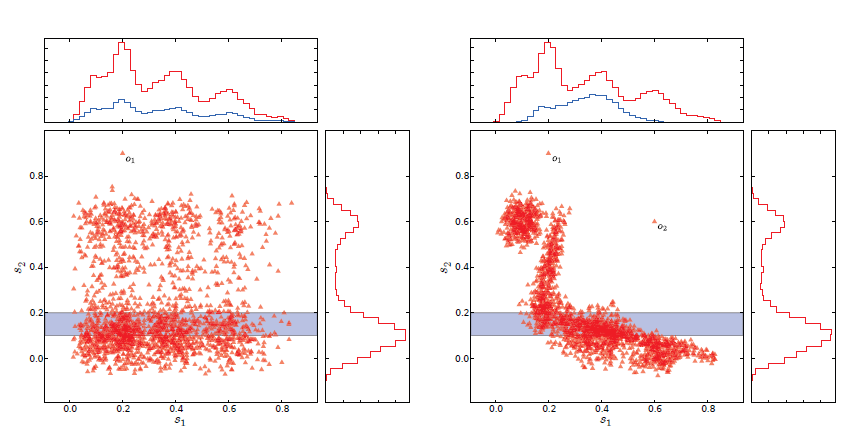
\includegraphics[scale=0.5]{Imagenes/ejemplo_anomalia_probabilidad}
\end{figure}

\end{frame}

\section{Modelos implementados}

\begin{frame}[fragile]{Algoritmos de Ensamblaje}
\vspace{10px}
\pause
\metroset{block=fill}

\begin{block}{Algoritmos de ensamblaje}
	\begin{itemize}
		\item Algoritmos secuenciales
		\pause
		\item Algoritmos independientes
	\end{itemize}
\end{block}

\pause

\begin{figure}
	\centering
	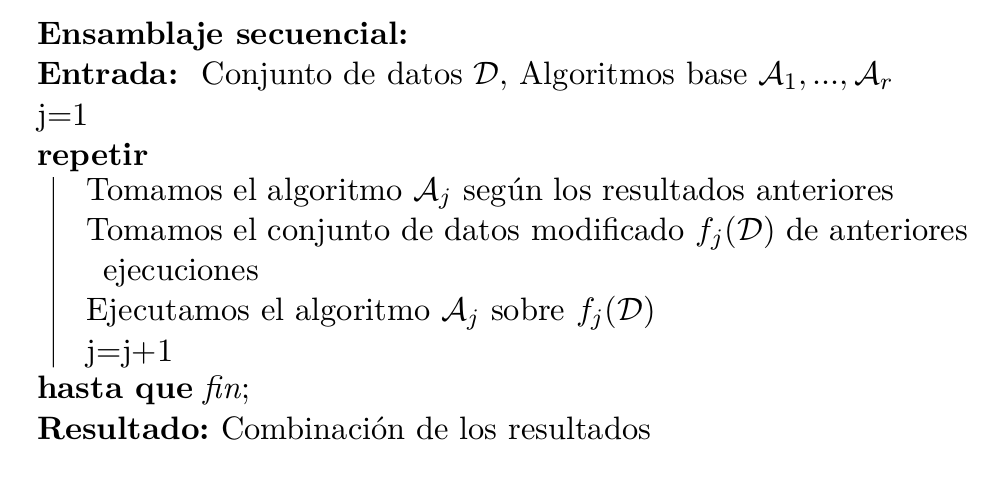
\includegraphics[scale=0.3]{Imagenes/ensamblaje-secuencial}
\end{figure}

\end{frame}

\begin{frame}[fragile]{Algoritmos de Ensamblaje}
\vspace{10px}
\metroset{block=fill}

\begin{block}{Algoritmos de ensamblaje}
	\begin{itemize}
		\item Algoritmos secuenciales

		\item Algoritmos independientes
	\end{itemize}
\end{block}

\begin{figure}
	\centering
	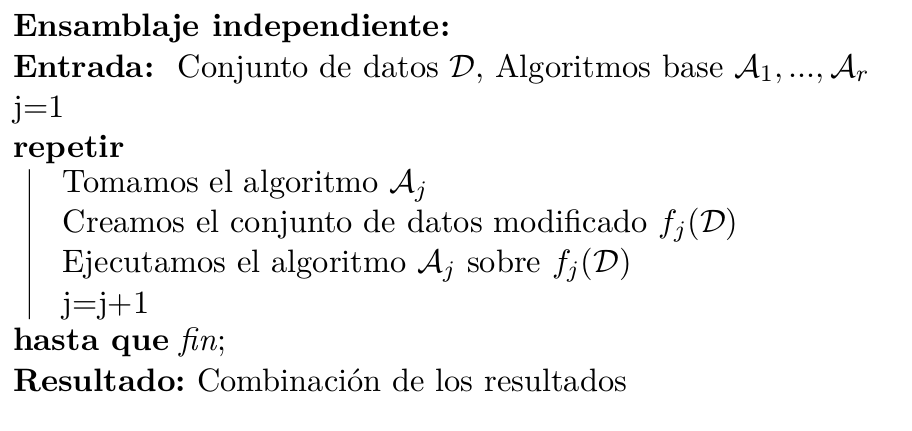
\includegraphics[scale=0.3]{Imagenes/ensamblaje-independiente}
\end{figure}

\end{frame}

\begin{frame}[fragile]{HICS}
\vspace{10px}
\pause
\metroset{block=fill}

\begin{algorithm}[H]{\textbf{HICS}}
	
	\KwIn{D: dataset}
	
	$scores = [ \ ]$
	
	$sub = $ subespacios de alto contraste
	
	\ForEach{$S \in sub$}{
		
		Ajustamos un modelo con el algoritmo LOF con la proyección sobre $S$
		
		$scores = scores + puntaje \ LOF$
		
	}
	
	$scores = \frac{scores}{|sub|}$
	
	\KwOut{scores: puntajes}
	
\end{algorithm}

\end{frame}

\begin{frame}[fragile]{HICS}
\vspace{10px}
\pause
\metroset{block=fill}

\begin{algorithm}[H]{\textbf{CalcularConstraste}}
	
	\KwIn{subespacio: subespacio, M: número de iteraciones del subsampling, $\alpha$: valor para obtener el tamaño de la muestra, $D$: conjunto de datos}
	
	$size = n \cdot \sqrt[|subespacio|]{\alpha}$
	
	$dev=0$
	
	\ForEach{$i\in [1,M]$}{
		
		$comp\_atr = aleatorio \ de \ subespacio$
		
		$sel\_obj = $ muestra aleatoria de $D$ de tamaño $size$
		
		$dev = dev + CalcularDev(comp\_atr, sel\_obj, subespacio, D)$
		
	}
	
	$dev = \frac{dev}{M}$
	
	\KwOut{$dev$: contraste}
	
\end{algorithm}

\end{frame}

\begin{frame}[fragile]{HICS}
\vspace{10px}
\pause
\metroset{block=fill}

\begin{algorithm}[H]{\textbf{CalcularDev}}
	
	\KwIn{$comp\_atr$: atributo con el que comparar, $sel\_obj$: muestra seleccionada aleatoriamente, $subespacio$: subespacio sobre el que calcular la desviación, $D$: conjunto de datos}
	
	$max = 0$
	
	\ForEach{$d\in D$}{
		
		$cum_1 = \sum_{o\in D} o[comp\_atr]$ si $o[comp\_atr]<d[comp\_atr]$
		
		$cum_2 = \sum_{o\in sel\_obj} o[comp\_atr]$ si $o[comp\_atr]<d[comp\_atr]$
		
		$f_a = \frac{cum_1}{|D|}$
		
		$f_b = \frac{cum_2}{|D|}$
		
		$subs = |f_a - f_b|$
		
		\If{$subs>max$}{
			
			$max = subs$
			
		}
		
	}
	
	\KwOut{max: máxima desviación}
	
\end{algorithm}

\end{frame}

\begin{frame}[fragile]{OUTRES}
\vspace{10px}
\pause
\metroset{block=fill}

\begin{algorithm}[H]
	
	\KwIn{o: instancia, S: subespacio}
	
	\ForEach{$i\in (D \setminus S)$}{
		
		$S' = S\cup \{ i \}$
		
		\If{$S'$ es relevante}{
			
			$den(o, S') = \frac{1}{n} \sum_{p\in AN(o,S')} K_e (\frac{dist_{S'}(o,p)}{\epsilon (|S'|)})$
			
			$dev(o,S') = \frac{\mu - den(o,S')}{2\sigma}$
			
			\If{$dev(o,S')\geq 1$}{
				
				$r(o) = r(o) \cdot \frac{den(o,S')}{dev(o,S')}$
				
			}
			
			$OUTRES(o,S')$
			
		}
		
		\Else{
			
			Para recursividad
			
		}
		
	}
	
	\KwOut{r: puntajes}
	
\end{algorithm}

\end{frame}

\begin{frame}[fragile]{OUTRES}
\vspace{10px}
\pause
\metroset{block=fill}

\begin{block}{Subespacio relevante}
	Decimos que un subespacio es relevante si no está distribuido uniformemente.
\end{block}

\pause

\begin{alertblock}{Procedimiento}
	Si la proyección de los datos sobre un subespacio está distribuida según una uniforme entonces sus proyecciones en una dimensión también lo están.
\end{alertblock}

\end{frame}

\begin{frame}[fragile]{OUTRES}
\vspace{10px}
\pause
\metroset{block=fill}

\begin{block}{Elementos involucrados}
	$$AN(o,S) = \{ p | dist_{S}(o,p)\leq \epsilon (|S|) \}$$
	
	\pause
	
	$$\epsilon (|S|) = 0.5 \cdot \frac{h_{optimal}(|S|)}{h_{optimal}(2)}$$
	
	\pause
	
	$$h_{optimal} (d) = (\frac{8\Gamma (\frac{d}{2} + 1)}{\pi^{\frac{d}{2}}}(d+4)(2\sqrt{\pi})^d) n^{\frac{-1}{d+4}}$$
	
	\pause
	
	$$K_{\epsilon}(x) = (1-x^2) \ \forall x<1$$
\end{block}

\end{frame}

\begin{frame}[fragile]{LODA}
\vspace{10px}
\pause
\metroset{block=fill}

\begin{algorithm}[H]{\textbf{ProyeccionesAleatorias}}
	
	\KwIn{$d$: dimension, $D$: dataset, $k$: número de histogramas y proyecciones}
	
	$no\_neg = [\sqrt{d}]$
	
	$proyecciones = [ \ ]$
	
	\ForEach{$i\in [1,k]$}{
		
		$ind = $ $no\_neg$ indices aleatorios en $[0,d]$
		
		$proy = $ vector con ceros en todas las posiciones menos en ind, donde hay valores sacados de una normal $\mathcal{N}(0,1)$
		
		$proyecciones = [proecciones, proy]$
		
	}
	
	\KwOut{$proyecciones$: proyecciones}
	
\end{algorithm}

\end{frame}

\begin{frame}[fragile]{LODA}
\vspace{10px}
\pause
\metroset{block=fill}

\begin{algorithm}[H]{\textbf{ObtenerHistogramas}}
	
	\KwIn{$D$: dataset, $\{w_i\}_{i=1}^{k}$: vectores de proyecciones, $k$: numero de histogramas y vectores de proyección}
	
	Inicializamos los histogramas $\{h_i\}_{i=1}^{k}$
	
	\For{$j=1 \rightarrow |D|$}{
		
		\For{$i=1\rightarrow k$}{
			
			$z_i = x_j^T w_i$	
			
			Actualiza el histograma $h_i$ con $z_i$
			
		}
		
	}
	
	\KwOut{$\{h_i\}_{i=1}^{k}$: histogramas}
	
\end{algorithm}

\end{frame}

\begin{frame}[fragile]{LODA}
\vspace{10px}
\pause
\metroset{block=fill}

\begin{algorithm}[H]{\textbf{LODA}}
	
	\KwIn{$x$: instancia, $\{h_i\}_{i=1}^{k}$: histogramas, $\{w_i\}_{i=1}^{k}$: vectores de proyección}
	
	\For{$i=1\rightarrow k$}{
		
		$z_i = x^T w_i$
		
		Obtenemos $p_i = p_i (z_i)$ del histograma $h_i$
		
	}
	
	$f = \frac{-1}{k} \sum_{i=1}^{k}\log (p_i (z_i))$
	
	\KwOut{$f$: puntaje de anomalía de $x$}
	
\end{algorithm}

\end{frame}

\begin{frame}[fragile]{Mahalanobis Kernel}
\vspace{10px}
\pause
\metroset{block=fill}

\begin{algorithm}[H]{\textbf{Mahalanobis Kernel}}
	\KwIn{$D$}
	
	$S = DD^T$.
	
	$S = Q\Delta^2 Q^T$.
	
	Almacenamos los vectores propios columna no negativos de $Q\Delta$ en una matriz $D'$
	
	Normalizamos $D'$ para que tenga media $0$ y varianza $1$.
	
	$vector\_media = media(D')$
	
	$puntuaciones = []$
	
	\ForEach{fila en D'}{
		$score = distancia(vector\_media , fila)$
		
		$puntuaciones = [puntuaciones, score]$
	}
	\KwOut{puntuaciones}
\end{algorithm}

\end{frame}

\begin{frame}[fragile]{Trinity}
\vspace{10px}
\pause
\metroset{block=fill}


\begin{block}{Componentes}
	\begin{enumerate}
		\item Componente basado en distancias: KNN con $k=5$
		\pause
		\item Componente basado en dependencia: Mahalanobis Kernel
		\pause
		\item Componente basado en densidad en subespacios: IForest
	\end{enumerate}
\end{block}

\begin{alertblock}
	Aplicamos en todos los componentes la técnica de subsampling.
\end{alertblock}

\end{frame}

\begin{frame}[fragile]{Trinity}
\vspace{10px}
\pause
\metroset{block=fill}

\begin{algorithm}[H]{\textbf{Trinity}}
	\KwIn{$D$}
	
	Ejecutamos KNN con $k=5$ y guardamos el resultado en $E_1$
	
	Ejecutamos Mahalanobis Kernel y guardamos el resultado en $E_2$
	
	Ejecutamos IForest y guardamos el resultado en $E_3$
	
	Estandarizamos $E_1 , E_2 \ y \ E_3$ a media $0$ y varianza $1$
	
	Hacemos la media para obtener las puntuaciones
	
	\KwOut{puntuaciones}
\end{algorithm}

\end{frame}

\begin{frame}[fragile]{Implementación}
\vspace{10px}
\pause
\metroset{block=fill}

\begin{block}{Recursos usados}
	\begin{itemize}
		\item Implementación hecha en Python3
		\pause
		\item Disponible en GitHub
		\pause
		\item Documentada con Sphinx
	\end{itemize}
\end{block}

\end{frame}

\section{Resultados}

\begin{frame}[fragile]{Conversión del problema a semisupervisado}
\vspace{10px}
\pause
\metroset{block=fill}

\begin{alertblock}{Problema}
	Si queremos medir el rendimiento de los modelos necesitamos conjuntos de datos que tengan detectadas las anomalías.
\end{alertblock}

\pause

\begin{alertblock}{Solución}
	Vamos a utilizar los conjuntos de datos de ODDS de la Universidad de Stony Brooks.
\end{alertblock}

\end{frame}

\begin{frame}[fragile]{Conjuntos de datos ODDS}
\vspace{10px}
\pause
\metroset{block=fill}

\begin{block}{Problema}
	Conjuntos de datos mantenidos por la Universidad Stony Brooks. Etiquetados los datos con 0 si son normales y 1 si son anomalías.
\end{block}

\end{frame}

\begin{frame}[fragile]{Conjuntos de datos ODDS}
\vspace{10px}
\pause
\metroset{block=fill}

\begin{table}[H]
	\centering
	\begin{tabular}{|l|l|l|}
		\hline
		\multicolumn{1}{|c|}{{\ul Nombre}} & \multicolumn{1}{c|}{{\ul Dimensionalidad}} & \multicolumn{1}{c|}{{\ul Número de instancias}} \\ \hline
		annthyroid                                  & 6                                                   & 7200                                                     \\ \hline
		arrhythmia                                  & 274                                                 & 452                                                      \\ \hline
		breastw                                     & 9                                                   & 683                                                      \\ \hline
		cardio                                      & 21                                                  & 1831                                                     \\ \hline
		glass                                       & 9                                                   & 214                                                      \\ \hline
		ionosphere                                  & 33                                                  & 351                                                      \\ \hline
		letter                                      & 32                                                  & 1600                                                     \\ \hline
		lympho                                      & 18                                                  & 148                                                      \\ \hline
		mammography                                 & 6                                                   & 11183                                                    \\ \hline
		mnist                                       & 100                                                 & 7603                                                     \\ \hline
		musk                                        & 166                                                 & 3062                                                     \\ \hline
		optdigits                                   & 64                                                  & 5216                                                     \\ \hline
		pendigits                                   & 16                                                  & 6870                                                     \\ \hline
		pima                                        & 8                                                   & 768                                                      \\ \hline
	\end{tabular}
\end{table}

\end{frame}

\begin{frame}[fragile]{Conjuntos de datos ODDS}
\vspace{10px}
\metroset{block=fill}

\begin{table}[H]
	\centering
	\begin{tabular}{|l|l|l|}
		\hline
		\multicolumn{1}{|c|}{{\ul Nombre}} & \multicolumn{1}{c|}{{\ul Dimensionalidad}} & \multicolumn{1}{c|}{{\ul Número de instancias}} \\ \hline
		satellite                                   & 36                                                  & 6435                                                     \\ \hline
		satimage-2                                  & 36                                                  & 5803                                                     \\ \hline
		speech                                      & 400                                                 & 3686                                                     \\ \hline
		thyroid                                     & 6                                                   & 3772                                                     \\ \hline
		vertebral                                   & 6                                                   & 240                                                      \\ \hline
		vowels                                      & 12                                                  & 1456                                                     \\ \hline
		wbc                                         & 30                                                  & 378                                                      \\ \hline
		wine                                        & 13                                                  & 129                                                      \\ \hline
	\end{tabular}
\end{table}

\end{frame}

\begin{frame}[fragile]{Modelos PyOD}
\vspace{10px}
\metroset{block=fill}

\begin{block}{Experimentación}
	Los 5 modelos se han puesto frente a modelos clásicos implementados en la librería PyOD.
	
	\pause
	
	Angle-Based Outlier Detection (ABOD), Connectivity-Based Outlier Factor (COF), Histogram-Based Outlier Score (HBOS), K Nearest Neighbors (KNN), Local Outlier Factor (LOF), Minimum Covariance Determinant (MCD), One-Class Support Vector Machines (OCSVM), Principal Component Analysis (PCA), Subspace Outlier Detection (SOD) y Stochastic Outlier Selection (SOS)
\end{block}

\end{frame}

\begin{frame}[fragile]{Acierto}
\vspace{10px}
\metroset{block=fill}

\begin{alertblock}{Mejores modelos}
	Trinity, Mahalanobis Kernel y LODA
\end{alertblock}

\pause

\begin{alertblock}{Peores modelos}
	HICS y OUTRES
\end{alertblock}

\end{frame}

\begin{frame}[fragile]{Dificultad del problema}
\vspace{10px}
\metroset{block=fill}

\begin{figure}
	\centering
	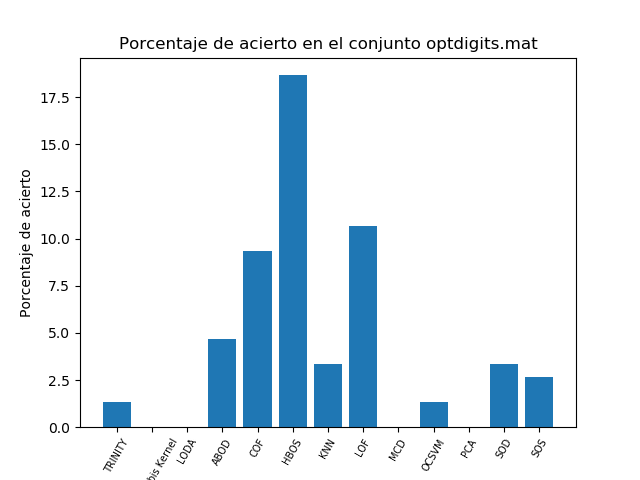
\includegraphics[scale=0.6]{Imagenes/optdigits-score}
\end{figure}

\end{frame}

\begin{frame}[fragile]{Buenos resultados}
\vspace{10px}
\metroset{block=fill}

\begin{figure}
	\centering
	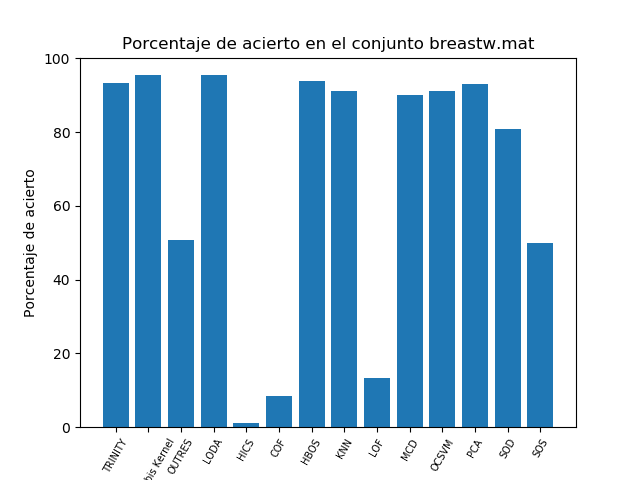
\includegraphics[scale=0.6]{Imagenes/breastw-score}
\end{figure}

\end{frame}

\begin{frame}[fragile]{Mejor resultado de HICS}
\vspace{10px}
\metroset{block=fill}

\begin{figure}
	\centering
	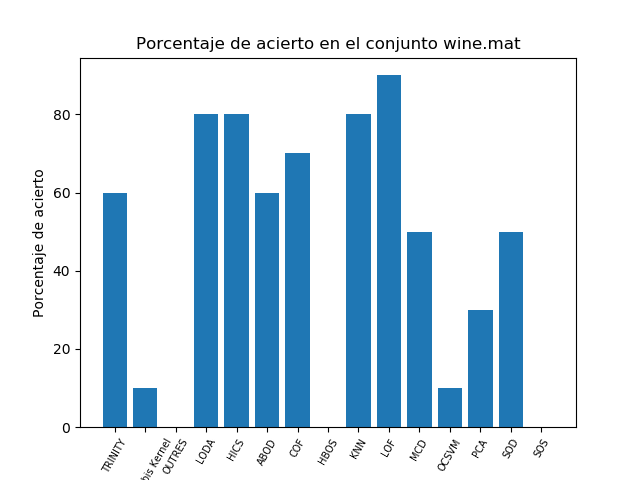
\includegraphics[scale=0.6]{Imagenes/wine-score}
\end{figure}

\end{frame}

\begin{frame}[fragile]{Porcentaje de acierto}
\vspace{10px}
\metroset{block=fill}

\begin{table}
	\resizebox{\textwidth}{!}{
	\begin{tabular}{|c|c|c|c|c|c|} 
		\hline
		\textbf{Data / Mod}  & \textbf{Trinity}    & \textbf{MK}         & \textbf{OUTRES}  & \textbf{LODA}       & \textbf{HICS}   \\ 
		\hline
		\textbf{annthyroid}   & 26.2172\%           & 12.3595\%           & 7.4906\%         & 8.9887\%            & 6.5543\%        \\ 
		\hline
		\textbf{arrhythmia}   & 48.4848\%           & \textbf{51.5151\%}  & NAN              & 37.8787\%           & NAN             \\ 
		\hline
		\textbf{breastw}      & 93.3054\%           & \textbf{95.3974\%}  & 50.6276\%        & \textbf{95.3974}    & 1.2552\%        \\ 
		\hline
		\textbf{cardio}       & 44.3181\%           & 51.7045\%           & NAN              & 59.0909\%           & NAN             \\ 
		\hline
		\textbf{glass}        & 11.1111\%           & 0\%                 & 0\%              & 0\%                 & 11.1111\%       \\ 
		\hline
		\textbf{ionosphere}   & 73.0158\%           & 57.1428\%           & NAN              & 46.8253\%           & NAN             \\ 
		\hline
		\textbf{letter}       & 16\%                & 15\%                & NAN              & 4\%                 & NAN             \\ 
		\hline
		\textbf{lympho}       & 83.3333\%           & 50\%                & NAN              & 0\%                 & NAN             \\ 
		\hline
		\textbf{mammography}  & 25.7692\%           & 1.1538\%            & 5.3846\%         & \textbf{28.0769\%}  & 8.0769\%        \\ 
		\hline
		\textbf{mnist}        & 40.2857\%           & \textbf{54.7142\%}  & NAN              & 2\%                 & NAN             \\ 
		\hline
		\textbf{musk}         & 34.0206\%           & 0\%                 & NAN              & 32.9896\%           & NAN             \\ 
		\hline
		\textbf{optdigits}    & 1.3333\%            & 0\%                 & NAN              & 0\%                 & NAN             \\ 
		\hline
		\textbf{pendigits}    & 25\%                & 16.6666\%           & 2.5641\%         & 0\%                 & NAN             \\ 
		\hline
		\textbf{pima}         & 50.7462\%           & 38.8059\%           & 34.7014\%        & \textbf{54.8507\%}  & 30.5970\%       \\ 
		\hline
	\end{tabular}
}
\end{table}

\end{frame}

\begin{frame}[fragile]{Porcentaje de acierto}
\vspace{10px}
\metroset{block=fill}

\begin{table}
	\resizebox{\textwidth}{!}{
	\begin{tabular}{|c|c|c|c|c|c|} 
		\hline
		\textbf{Data / Mod}  & \textbf{Trinity}    & \textbf{MK}         & \textbf{OUTRES}  & \textbf{LODA}       & \textbf{HICS}   \\ 
		\hline
		\textbf{satellite}    & 54.3713\%           & 32.8585\%           & NAN              & 12.6227\%           & NAN             \\ 
		\hline
		\textbf{satimage-2}   & \textbf{90.1408\%}  & \textbf{90.1408\%}  & NAN              & 0\%                 & NAN             \\ 
		\hline
		\textbf{speech}       & 0\%                 & 4.9180\%            & NAN              & 3.2786\%            & NAN             \\ 
		\hline
		\textbf{thyroid}      & 39.7849\%           & 22.5806\%           & 5.3763\%         & 1.0752\%            & 0\%             \\ 
		\hline
		\textbf{vertebral}    & 3.3333\%            & 10\%                & 3.3333\%         & 0\%                 & 3.3333\%        \\ 
		\hline
		\textbf{vowels}       & 24\%                & 0\%                 & 4\%              & 8\%                 & 32\%            \\ 
		\hline
		\textbf{wbc}          & 42.8571\%           & 0\%                 & NAN              & \textbf{71.4285\%}  & NAN             \\ 
		\hline
		\textbf{wine}         & 60\%                & 10\%                & 0\%              & 80\%                & 80\%            \\
		\hline
	\end{tabular}
}
\end{table}

\end{frame}

\begin{frame}[fragile]{Proyecciones}
\vspace{10px}
\metroset{block=fill}

\begin{figure}
	\centering
	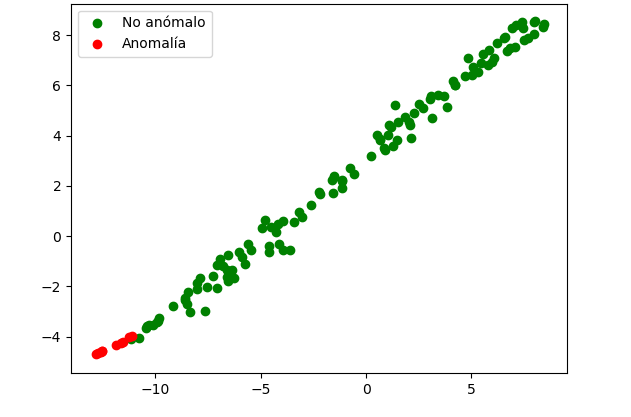
\includegraphics[scale=0.6]{Imagenes/wine}
	\caption*{Proyección del conjunto wine}
\end{figure}

\end{frame}

\begin{frame}[fragile]{Proyecciones}
\vspace{10px}
\metroset{block=fill}

\begin{figure}
	\centering
	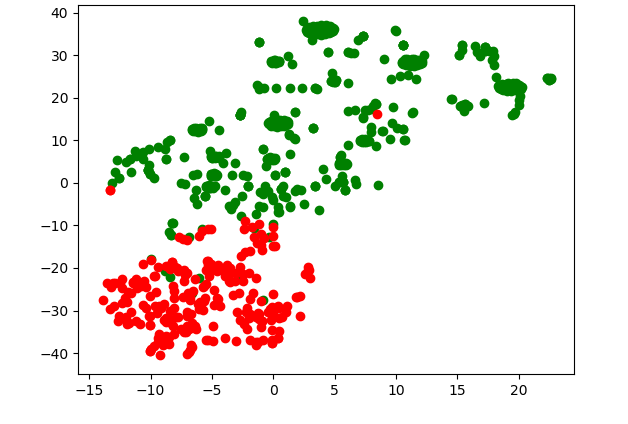
\includegraphics[scale=0.6]{Imagenes/breastw}
	\caption*{Proyección del conjunto breastw}
\end{figure}

\end{frame}

\begin{frame}[fragile]{Proyecciones}
\vspace{10px}
\metroset{block=fill}

\begin{figure}
	\centering
	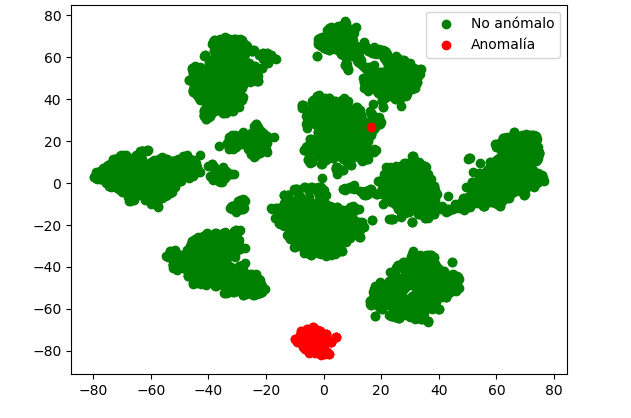
\includegraphics[scale=0.6]{Imagenes/optdigits}
	\caption*{Proyección del conjunto optdigits}
\end{figure}

\end{frame}

\begin{frame}[fragile]{OUTRES}
\vspace{10px}
\metroset{block=fill}

\begin{figure}
	\centering
	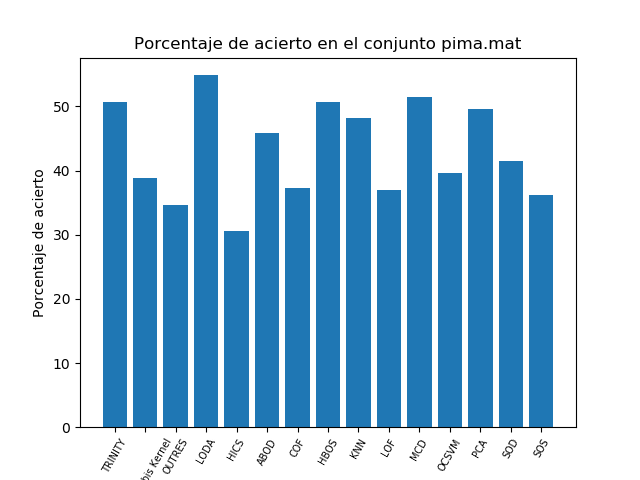
\includegraphics[scale=0.6]{Imagenes/pima-score}
\end{figure}

\end{frame}

\begin{frame}[fragile]{OUTRES}
\vspace{10px}
\metroset{block=fill}

\begin{figure}
	\centering
	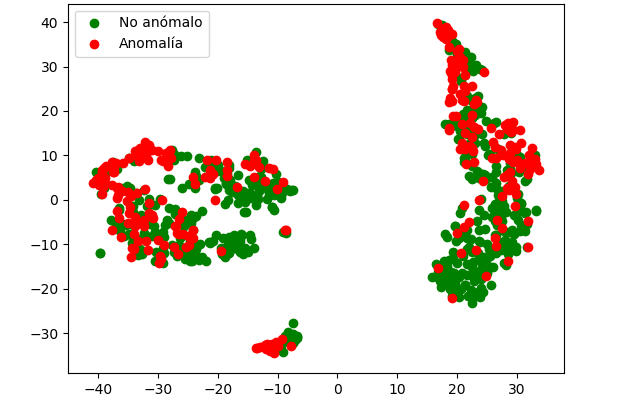
\includegraphics[scale=0.6]{Imagenes/pima}
	\caption*{Proyección del conjunto pima}
\end{figure}

\end{frame}

\begin{frame}[fragile]{OUTRES}
\vspace{10px}
\metroset{block=fill}

\begin{figure}
	\centering
	\begin{subfigure}{0.49\textwidth}
		\centering
		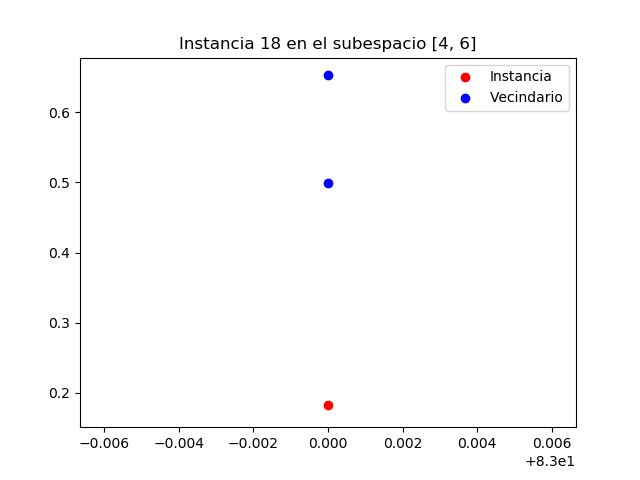
\includegraphics[scale=0.36]{Imagenes/22}
	\end{subfigure}
	\pause
	\begin{subfigure}{0.49\textwidth}
		\centering
		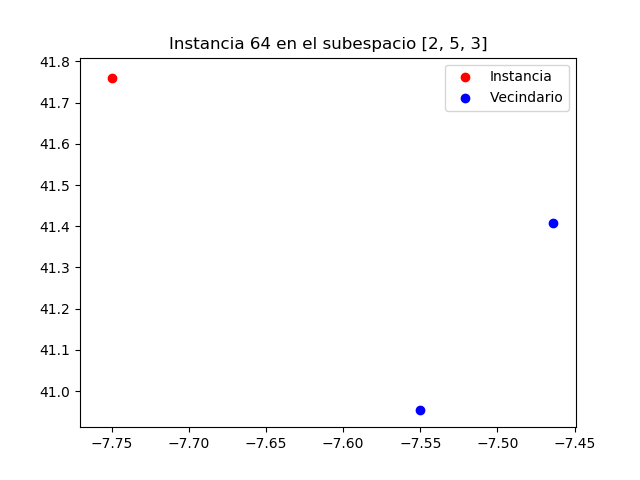
\includegraphics[scale=0.36]{Imagenes/68-tsne}
	\end{subfigure}
\end{figure}

\end{frame}

\begin{frame}[fragile]{OUTRES}
\vspace{10px}
\metroset{block=fill}

\begin{figure}
	\centering
	\begin{subfigure}{0.49\textwidth}
		\centering
		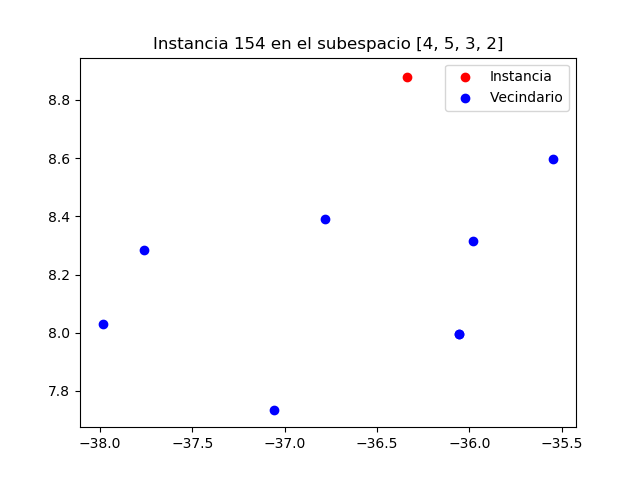
\includegraphics[scale=0.36]{Imagenes/173-tsne}
	\end{subfigure}
	\pause
	\begin{subfigure}{0.49\textwidth}
		\centering
		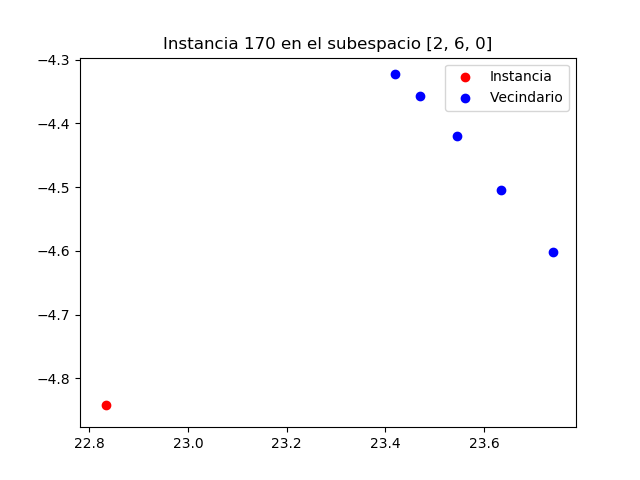
\includegraphics[scale=0.36]{Imagenes/190-tsne}
	\end{subfigure}
\end{figure}

\end{frame}

\begin{frame}[fragile]{AUC y ROC}
\vspace{10px}
\metroset{block=fill}

\begin{block}{Valores AUC}
	$$TPR = \frac{VP}{VP + FN}, \ FPR = \frac{FP}{VN + FP}$$
	
	\pause
	
	Área bajo la curva
\end{block}

\end{frame}

\begin{frame}[fragile]{AUC y ROC}
\vspace{10px}
\metroset{block=fill}

\begin{table}
	\centering
	\begin{tabular}{|c|c|c|c|c|c|} 
		\hline
		\textbf{Data / Model}  & \textbf{Tinity}  & \textbf{MK}      & \textbf{OUTRES}  & \textbf{LODA}    & \textbf{HICS}   \\ 
		\hline
		\textbf{annthyroid}     & 0.6015           & 0.5266           & 0.5003           & 0.5084           & 0.4953          \\ 
		\hline
		\textbf{arrhythmia}     & 0.6983           & \textbf{0.7161}  & NAN              & 0.6362           & NAN             \\ 
		\hline
		\textbf{breastw}        & 0.9485           & \textbf{0.9646}  & 0.6202           & \textbf{0.9646}  & 0.2405          \\ 
		\hline
		\textbf{cardio}         & 0.6919           & 0.7328           & NAN              & 0.7737           & NAN             \\ 
		\hline
		\textbf{glass}          & 0.5360           & 0.4780           & 0.4780           & 0.4780           & 0.5360          \\ 
		\hline
		\textbf{ionosphere}     & 0.7895           & 0.6657           & NAN              & 0.5852           & NAN             \\ 
		\hline
		\textbf{letter}         & 0.5519           & 0.5466           & NAN              & 0.488            & NAN             \\ 
		\hline
		\textbf{lympho}         & \textbf{0.9131}  & 0.7394           & NAN              & 0.4788           & NAN             \\ 
		\hline
		\textbf{mammography}    & 0.6200           & 0.4940           & 0.5156           & \textbf{0.6318}  & 0.5294          \\ 
		\hline
		\textbf{mnist}          & 0.6711           & \textbf{0.7506}  & NAN              & 0.4603           & NAN             \\ 
		\hline
		\textbf{musk}           & 0.6593           & 0.4836           & NAN              & 0.6539           & NAN             \\ 
		\hline
		\textbf{optdigits}      & 0.4920           & 0.4851           & NAN              & 0.4851           & NAN             \\ 
		\hline
		\textbf{pendigits}      & 0.6162           & 0.5736           & 0.5015           & 0.4883           & NAN             \\ 
		\hline
		\textbf{pima}           & 0.6217           & 0.5300           & 0.4985           & \textbf{0.6532}  & 0.4669          \\ 
		\hline
	\end{tabular}
\end{table}

\end{frame}

\begin{frame}[fragile]{AUC y ROC}
\vspace{10px}
\metroset{block=fill}

\begin{table}
	\centering
	\begin{tabular}{|c|c|c|c|c|c|} 
		\hline
		\textbf{Data / Model}  & \textbf{Tinity}  & \textbf{MK}      & \textbf{OUTRES}  & \textbf{LODA}    & \textbf{HICS}   \\ 
		\hline
		\textbf{satellite}      & 0.6662           & 0.5089           & NAN              & 0.3609           & NAN             \\ 
		\hline
		\textbf{satimage-2}     & \textbf{0.9500}  & \textbf{0.9500}  & NAN              & 0.4938           & NAN             \\ 
		\hline
		\textbf{speech}         & 0.4915           & 0.5165           & NAN              & 0.5082           & NAN             \\ 
		\hline
		\textbf{thyroid}        & 0.6913           & 0.6031           & 0.5149           & 0.4928           & 0.4873          \\ 
		\hline
		\textbf{vertebral}      & 0.4476           & 0.4857           & 0.4476           & 0.4285           & 0.4476          \\ 
		\hline
		\textbf{vowels}         & 0.6064           & 0.4822           & 0.5029           & 0.5236           & 0.6479          \\ 
		\hline
		\textbf{wbc}            & 0.6974           & 0.4705           & NAN              & \textbf{0.8487}  & NAN             \\ 
		\hline
		\textbf{wine}           & 0.7831           & 0.5121           & 0.4579           & 0.8915           & 0.8915          \\
		\hline
	\end{tabular}
\end{table}

\end{frame}

\begin{frame}[fragile]{AUC y ROC}
\vspace{10px}
\metroset{block=fill}

\begin{figure}[H]
	\centering
	\begin{subfigure}{.49\textwidth}
		\centering
		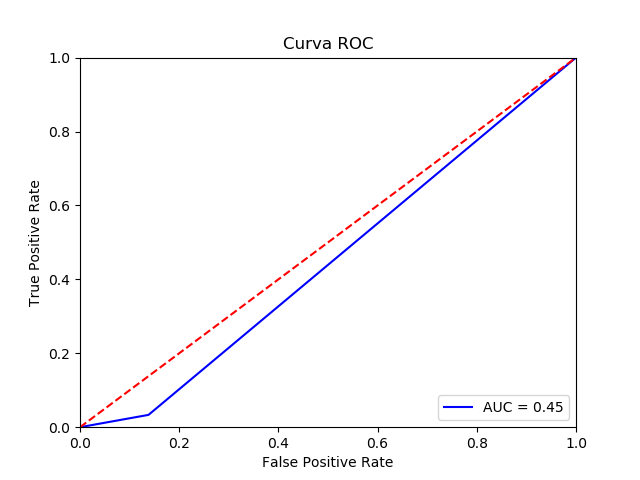
\includegraphics[scale=0.35]{Imagenes/roc/TRINITY_vertebral}
	\end{subfigure}
	\begin{subfigure}{.49\textwidth}
		\centering
		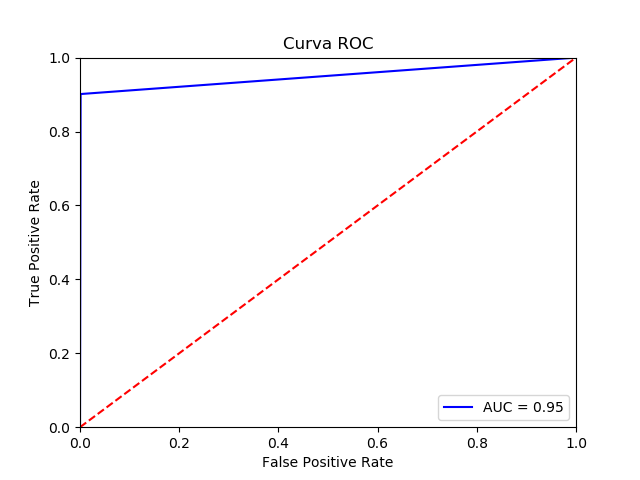
\includegraphics[scale=0.35]{Imagenes/roc/TRINITY_satimage-2}
	\end{subfigure}
	\caption*{Curvas ROC para Trinity}
	\label{ROC_TRINITY}
\end{figure}

\end{frame}

\begin{frame}[fragile]{AUC y ROC}
\vspace{10px}
\metroset{block=fill}

\begin{figure}[H]
	\centering
	\begin{subfigure}{.49\textwidth}
		\centering
		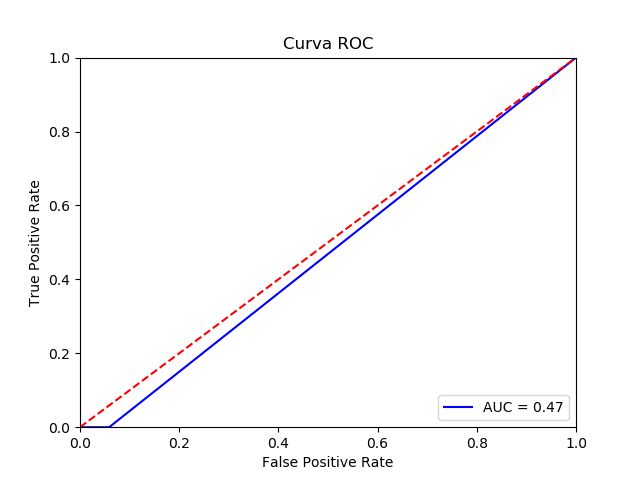
\includegraphics[scale=0.35]{Imagenes/roc/Mahalanobis_Kernel_wbc}
	\end{subfigure}
	\begin{subfigure}{.49\textwidth}
		\centering
		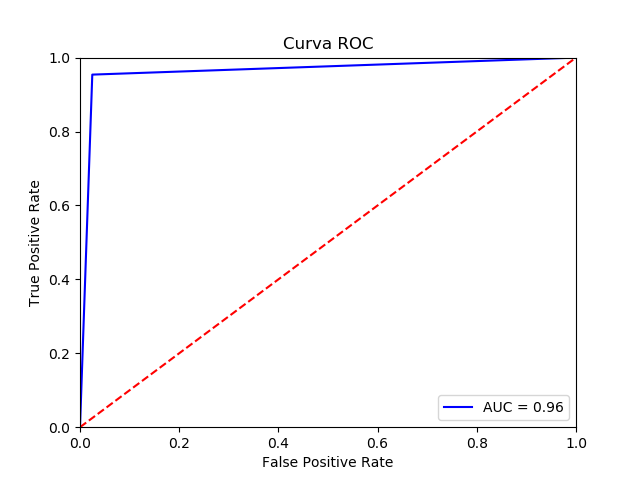
\includegraphics[scale=0.35]{Imagenes/roc/Mahalanobis_Kernel_breastw}
	\end{subfigure}
	\caption*{Curvas ROC para Mahalanobis Kernel}
	\label{ROC_MK}
\end{figure}

\end{frame}

\begin{frame}[fragile]{AUC y ROC}
\vspace{10px}
\metroset{block=fill}

\begin{figure}[H]
	\centering
	\begin{subfigure}{.49\textwidth}
		\centering
		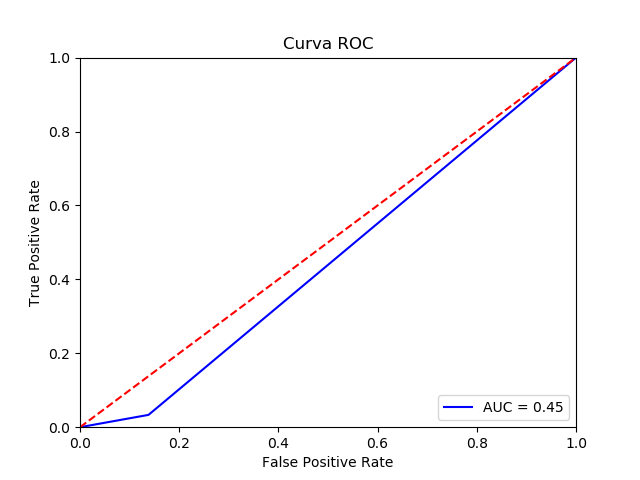
\includegraphics[scale=0.35]{Imagenes/roc/OUTRES_vertebral}
	\end{subfigure}
	\begin{subfigure}{.49\textwidth}
		\centering
		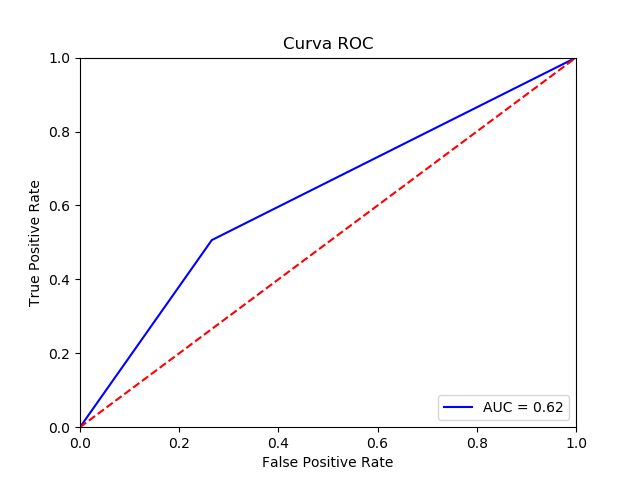
\includegraphics[scale=0.35]{Imagenes/roc/OUTRES_breastw}
	\end{subfigure}
	\caption*{Curvas ROC para OUTRES}
	\label{ROC_OUTRES}
\end{figure}

\end{frame}

\begin{frame}[fragile]{AUC y ROC}
\vspace{10px}
\metroset{block=fill}

\begin{figure}[H]
	\centering
	\begin{subfigure}{.49\textwidth}
		\centering
		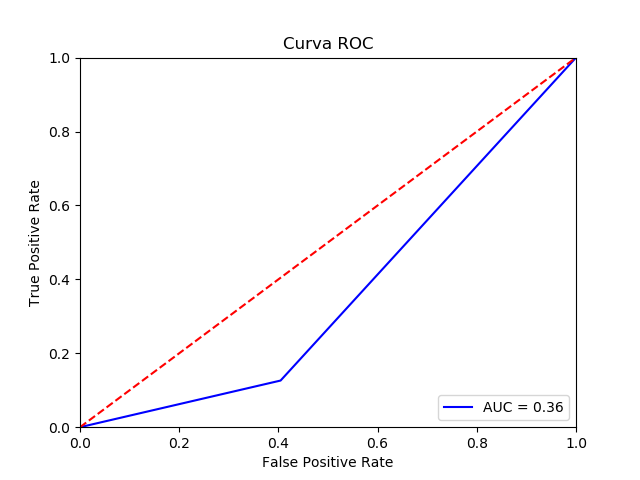
\includegraphics[scale=0.35]{Imagenes/roc/LODA_satellite}
	\end{subfigure}
	\begin{subfigure}{.49\textwidth}
		\centering
		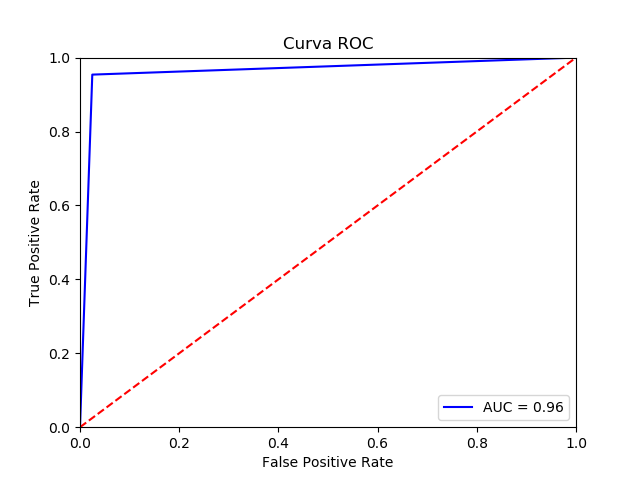
\includegraphics[scale=0.35]{Imagenes/roc/LODA_breastw}
	\end{subfigure}
	\caption*{Curvas ROC para LODA}
	\label{ROC_LODA}
\end{figure}

\end{frame}

\begin{frame}[fragile]{AUC y ROC}
\vspace{10px}
\metroset{block=fill}

\begin{figure}[H]
	\centering
	\begin{subfigure}{.49\textwidth}
		\centering
		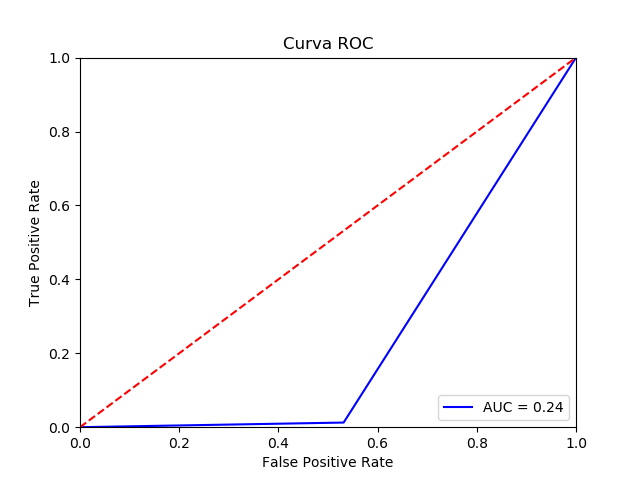
\includegraphics[scale=0.35]{Imagenes/roc/HICS_breastw}
	\end{subfigure}
	\begin{subfigure}{.49\textwidth}
		\centering
		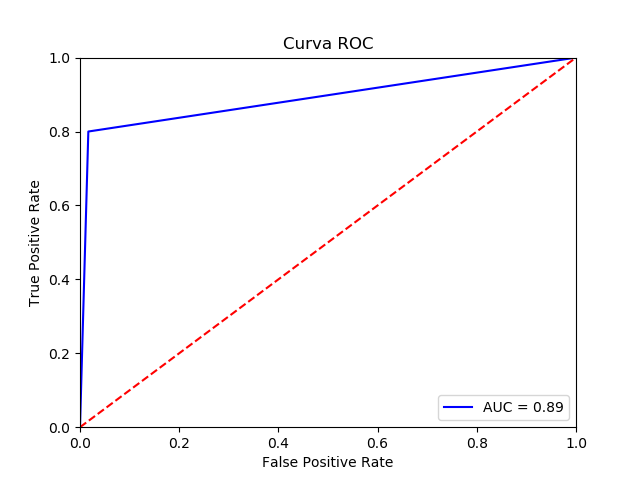
\includegraphics[scale=0.35]{Imagenes/roc/HICS_wine}
	\end{subfigure}
	\caption*{Curvas ROC para HICS}
	\label{ROC_HICS}
\end{figure}

\end{frame}

\begin{frame}[fragile]{Tiempos}
\vspace{10px}
\metroset{block=fill}

\begin{table}
	\resizebox{\textwidth}{!}{
	\begin{tabular}{|c|c|c|c|c|c|} 
		\hline
		\textbf{Data / Mod}  & \textbf{Trinity}  & \textbf{MK}  & \textbf{OUTRES}  & \textbf{LODA}  & \textbf{HICS}   \\ 
		\hline
		\textbf{annthyroid}   & 28.5212           & 390.5937     & 193.6110         & 137.8692       & 1169.3422       \\ 
		\hline
		\textbf{arrhythmia}   & 28.8828           & 0.1243       & NAN              & 9.0474         & NAN             \\ 
		\hline
		\textbf{breastw}      & 23.3296           & 0.3165       & 117.8225         & 13.2879        & 315.4130        \\ 
		\hline
		\textbf{cardio}       & 33.0496           & 6.5851       & NAN              & 36.6768        & NAN             \\ 
		\hline
		\textbf{glass}        & 12.5272           & 0.0220       & 11.5349          & 4.0798         & 79.2560         \\ 
		\hline
		\textbf{ionosphere}   & 16.5319           & 0.0565       & NAN              & 6.9664         & NAN             \\ 
		\hline
		\textbf{letter}       & 41.8301           & 5.1648       & NAN              & 31.8875        & NAN             \\ 
		\hline
		\textbf{lympho}       & 12.2874           & 0.0187       & NAN              & 2.8804         & NAN             \\ 
		\hline
		\textbf{mammography}  & 31.5619           & 1444.1323    & 27765.1978       & 224.8207       & 2502.0258       \\ 
		\hline
		\textbf{mnist}        & 42.7623           & 464.8962     & NAN              & 150.1434       & NAN             \\ 
		\hline
		\textbf{musk}         & 42.8683           & 34.4336      & NAN              & 60.4207        & NAN             \\ 
		\hline
		\textbf{optdigits}    & 36.2723           & 145.6876     & NAN              & 103.9115       & NAN             \\ 
		\hline
		\textbf{pendigits}    & 34.0999           & 340.2855     & 2757.0345        & 135.0839       & NAN             \\ 
		\hline
		\textbf{pima}         & 26.3576           & 0.3482       & 40.6379          & 15.2128        & 150.1283        \\ 
		\hline
	\end{tabular}
}
\end{table}

\end{frame}

\begin{frame}[fragile]{Tiempos}
\vspace{10px}
\metroset{block=fill}

\begin{table}
	\resizebox{\textwidth}{!}{
	\begin{tabular}{|c|c|c|c|c|c|} 
		\hline
		\textbf{Data / Mod}  & \textbf{Trinity}  & \textbf{MK}  & \textbf{OUTRES}  & \textbf{LODA}  & \textbf{HICS}   \\ 
		\hline
		\textbf{satellite}    & 48.2618           & 301.9960     & NAN              & 129.6712       & NAN             \\ 
		\hline
		\textbf{satimage-2}   & 39.7535           & 200.5037     & NAN              & 113.2818       & NAN             \\ 
		\hline
		\textbf{speech}       & 76.6633           & 62.2470      & NAN              & 73.0844        & NAN             \\ 
		\hline
		\textbf{thyroid}      & 32.6503           & 65.3469      & 64.2370          & 72.1607        & 376.2697        \\ 
		\hline
		\textbf{vertebral}    & 13.4726           & 0.0301       & 1.7653           & 4.6250         & 9.1404          \\ 
		\hline
		\textbf{vowels}       & 36.2093           & 3.1876       & 426.6157         & 28.2930        & 5126.5627       \\ 
		\hline
		\textbf{wbc}          & 17.0011           & 0.0675       & NAN              & 7.5109         & NAN             \\ 
		\hline
		\textbf{wine}         & 11.2756           & 0.0165       & 58.9642          & 2.4540         & 774.9212        \\
		\hline
	\end{tabular}
}
\end{table}

\end{frame}

\section{Conclusiones y Trabajo Futuro}

\begin{frame}[fragile]{Conclusiones y trabajo futuro}
\vspace{10px}
\metroset{block=fill}

\begin{block}{Conclusiones y trabajo futuro}
	\begin{itemize}
		\item Rendimiento similar a los clásicos aunque los superan en algunos casos: potencial.
		\pause
		\item Mal enfoque de los algoritmos HICS y OUTRES. Detección de anomalías no triviales.
		\pause
		\item Consumo de tiempo mucho mayor.
		\pause
		\item Valores perdidos y tratamiento.
		\pause
		\item Algoritmo nuevo.
	\end{itemize}
\end{block}

\end{frame}


\begin{frame}[standout]
	\LARGE{Gracias por su atención.}
	
	\vspace{10px}
	
	\LARGE{¿Preguntas?}
	\vspace{10px}
\end{frame}


\end{document}
